\chapter{Fejlesztői dokumentáció} % Developer guide
\label{ch:impl}

\section{A fejlesztői dokumentáció felépítése}

A 3.2 részben ismertetésre kerülnek a szoftver készítése során felhasznált technológiák, valamint nagy vonalakban a szoftver logikai felépítése. (Milyen programkomponensek vannak, milyen feladatokat látnak el, hogyan kapcsolódnak egymáshoz.) 

A 3.3-3.6 részek tartalmazzák az egyes komponensek részletesebb leírását. Minden komponens esetén ismertetésre kerül a más komponensek felé nyilvánosságra hozott interfész, valamint a komponensek működési elve, beleértve a használt típusok leírását és a fontosabb algoritmusok működési elvét. A rész sorrendileg úgy van felépítve, hogy először szerepelnek a vezérlő komponens (\textit{App}) által használt komponensek leírásai, majd ezt követően az \textit{App} moduljai. Így "lentről fölfelé" haladva először meg lehet érteni az egyes kisebb részek működését, majd azok segítségével az egész alkalmazásét.

A 3.7 rész tartalmazza a tesztelési eljárás leírását és a tesztelés eredményeit. 

\section{A szoftver felépítése}

\subsection{Felhasznált technológiák összefoglalása}

Az alkalmazás Haskell nyelven íródott. A grafikus megjelenítés \textit{GTK+} alapú, a \textit{gtk2hs} csomag által biztosított bindingokat használtam a grafikus felület kezeléséhez. Ez a csomag a \textit{GTK+} osztályhierarchiáját Haskell típusosztályok hierarchiájaként reprezentálja. Az egyes osztályok metódusainak a típusosztályok definíciójában szereplő függvények felelnek meg. A \textit{GTK+} típusai foreign pointerek segítségével vannak megvalósítva, és \textit{IO}-ban használhatók. 

Az alkalmazás a \textit{GTK+} logikájának megfelelően eseményvezérelt. A felhasználó akciói eseményeket váltanak ki, amelyek hatására esenénykezelők futnak le. A handlerek minden esetben \textit{IO} akciók, amelyek valamilyen módon módosítják a globális állapotot (lásd 3.2.2.). A szoftver fejlesztése során fontos volt, hogy minél kevesebb legyen az tisztátalan (impure), \textit{IO}-n belül elvégzett számítás. Igyekeztem a program logikájának minél nagyobb részét egy tiszta, nem monadikus környezetben megvalósítani. Így a számítások helyessége könnyebben tesztelhető/verifikálható, az eseménykezelők már keveset számolnak az \textit{IO}-ban.

Az alkalmazás a parseolási feladatokhoz a \textit{parsec} csomagot, a gráfok kezeléséhez az \textit{fgl} csomagot, a ghci futtatásához pedig a \textit{ghcid}  csomagot használja. A modell adatainak könnyebb kezeléséhez a \textit{microlens-platform} csomagot használtam, ami a jól ismert \textit{lens} \cite{lens} csomag egy kevesebb funkciót és kevesebb függőséget tartalmazó változata. A függőségek pontos listája elérhető a Felhasználói dokumentációban, illetve az egyes programkomponensek részletes leírásakor is említésre kerülnek a fontosabb felhasznált csomagok.

\subsection{A globális állapot}

Az alkalmazás fő felépítését egy az FP Complete blogján megjelent cikk \cite{readert} inspirálta. 
Az alkalmazás a globális (olvasható) állapotot a \textit{ReaderT} monád transzformer segítségével valósítja meg, az alkalmazás vezérlése így egy \textit{ReaderT Env IO} környezetben történik, ahol \textit{Env} a globális állapotot leíró adattípus. Fontos megjegyezni, hogy bár az \textit{Env} típus komponensei az inicializálás után sosem módosulhatnak, a mögöttes állapot még változhat, hiszen a komponensek módosítható referenciák. Ez hasonló a Java nyelvben használható konstans referencia koncepciójához: a referencia nem változhat, de a referált adat igen.

A fentebb referált cikk által inspirálva a (GUI komponensein kívüli) globális állapot egy \textit{StateT} transzformer helyett módosítható referenciákkal (\textit{IORef} és \textit{MVar}) kezeltetik. Ugyanis hiába tiszta; ha globálisan használjuk a \textit{StateT}-t, valójában -- a programlogika szintjén -- ugyanúgy egy globális, módosítható állapotot vezetünk be. Szintén egy szempont, hogy a \textit{GTK+} alapú \textit{GUI} miatt eleve szerepelnek módosítható referenciák (foreign pointer) a globális állapotban, így ez a probléma semmiképpen nem kerülhető el teljesen. Egy további érv a globális \textit{StateT} ellen, hogy egy nagyobb monad stack szükségszerűen bonyolítja a programot. A \textit{ReaderT IO} ellenben még kifejezetten könnyen kezelhető. A cikk konkurrenciához köthető problémákat is említ a \textit{StateT}-vel kapcsolatban. Ez a szoftver jelenlegi verziójában még nem olyan jelentős (lévén a mostani implementáció nagyon kis mértékben épít konkurrenciára). Azonban a jövőre nézve mindenképpen előnyös, ha a szoftvert könnyen lehet a konkurrens paradigma szerint bővíteni.

Ezen bevezető után tekintsük a globális állapot definícióját! Az alábbi típusdefiníció (deriving clause-okkal kiegészítve) az \textit{App.Types} modulban található:
\lstset{caption={Az Env típus}, label=src:hs}
\begin{lstlisting}[language={Haskell}, label=src:env]
data EvalConfig = EvalConfig { modules :: [String]
                             , paths :: [String]
                             }

data EvalControl = EvalControl { eGhci    :: MVar Ghci
                               , eCommand :: MVar String
                               , eResult  :: MVar (Either String [String])
                               , eConfig  :: MVar EvalConfig 
                               }

data SaveStatus = Saved | Modified

data File = File FilePath SaveStatus
  
data Env = Env { evalControl  :: EvalControl
               , gui          :: Gui
               , state        :: IORef Spreadsheet
               , file         :: IORef (Maybe File)
               }
\end{lstlisting}

Az \textit{evalControl} mező tartalmazza a kifejezések ghci-ban való kiértékeléséhez szükséges erőforrásokat. Az \textit{eConfig} mező tartalmazza a GHCi-hoz tartozó konfigurációs beállításokat. (Betöltött modulok listája, és a modulok keresési útvonalainak listája.) Az \textit{eGhci} mező tartalmazza a háttérben futó GHCi példányra való hivatkozást. Az \textit{eCommand} és az \textit{eResult} valósítják meg a kommunikációt a kiértékelést végző szál és az alkalmazás fő szála között. Az \textit{eCommand}-nak a fő szál a termelője, és a kiértékelő szál a fogyasztója, az \textit{eResult}-nak pedig fordítva.

A \textit{gui} mező tartalmazza a GUI komponenseit. A pontos típusdefiníció a GUI leírásánál szerepel (3.2.3).

A \textit{state} mező egy módosítható referencia, ami a számolótáblát reprezentáló, \textit{Spreadsheet} típusú adatot referálja. A \textit{file} adattag tartalmazza az éppen a táblázatkezelőbe betöltött fájl fontosabb adatait (fájl neve, és állapota), amennyiben van betöltve fájl. 

Az \textit{EvalConfig} típus példánya \textit{Generic} és \textit{Serialize} típusosztályoknak. Erre az adatok mentéséhez van szükség (lásd 3.6.).

\subsection{A GUI}

Az alábbi kódrészlet a GUI definíciója az \textit{App.Types} modulból:

\lstset{caption={A Gui típus}, label=src:gui}
\begin{lstlisting}[language={Haskell}]
data Menubar = Menubar { newButton :: Button
                       , saveButton :: Button
                       , loadButton :: Button
                       , modulesButton :: Button
                       , pathsButton :: Button }

data Gui = Gui { mainWindow     :: Window
               , logWindow      :: ScrolledWindow
               , log            :: TextBuffer
               , table          :: Table
               , entryKeys      :: [(Entry,(Int,Int))]
               , colButtonKeys  :: [(Button, Char)]
               , editor         :: Entry
               , commandLine    :: Entry
               , menu           :: Menubar }
\end{lstlisting}

A \textit{Gui} típus tartalmazza a Gui azon komponenseit, amelyekre szükség van az eseménykezelők hozzáadásakor. A \textit{mainWindow} komponens tartalmazza az alkalmazás fő ablakát. 

A számolótábla megjelenítése egy \textit{Table} segítségével történik. A cellákat a \textit{Table}-ben elhelyezett \textit{Entry}-k reprezentálják. Minden \textit{Entry}-hez egy \textit{(Int,Int)} kulcs is eltároltatik. Ez mutatja, hogy a tábla melyik pozíciójához tartozik az adott \textit{Entry}. Ez egy objektumorientált nyelvben megoldható lenne egy leszármazott widgettel (amelynek van egy extra mezője), azonban a \textit{gtk2hs} keretein belül ezt körülményes lett volna megoldani, így inkább a jelenlegi megoldást választottam. Az \textit{Entry}-kulcs párokat az \textit{entryKeys} mező tartalmazza. Az oszlopok tetején levő gombokat a \textit{colButtonKeys} mező tartalmazza. Ebben a mezőben az is el van tárolva, hogy melyik gombhoz melyik oszlop tartozik.

A grafikus felület alján található log egy \textit{ScrolledWindow}-ban elhelyezkedő \textit{TextView}. Magára a \textit{TextView}-ra nincs szükség, csak az általa használt \textit{TextBuffer}-re, ezért azt nem is tartalmazza a \textit{Gui}. Az editor és a parancssor egy-egy \textit{Entry}-vel vannak implementálva. A \textit{menu} komponens tartalmazza felső menüsoron elérhető gombokat. 

A GUI layout ennél alaposabb dokumentációja a 3.7.3 alfejezetben érhető el. 

\subsection{A cellaazonosítók reprezentációja}

A nézetben célszerű a táblázat celláit \textit{(Int,Int)} párokkal azonosítani (oszlop és sor száma). A számolótábla logikájában (gráfreprezentáció, ahol a csúcsok jelölik a cellákat, lásd 3.4.1) azonban a cellákat egész számokkal kell azonosítani. A konverzióhoz az \textit{(Int,Int)} típusra példányosítva lett az \textit{Enum} típusosztály. (Megjegyzés: félrevezető lehet egy párokra megadott \textit{Enum} példány. A kódban csak a \textit{fromEnum} és \textit{toEnum} függvények használatosak párokra a típusosztály függvényei közül. A jövőben valószínűleg az \textit{Enum} példány helyett csak a konverziós függvények lesznek definiálva és használva.)

A nézetben bármely cellához tartozó \textit{(Int,Int)} azonosító mindkét tagja nemnegatív. Az \textit{A0} cellához tartozik a \textit{(0,0)} azonosító. Az első komponens az oszlop sorszáma, a második a sorhoz tartozó sorszám. A megadott \textit{fromEnum} függvény leszűkítése egy $\mathbb{N} \times \mathbb{N} \rightarrow \mathbb{N}$ bijekció, így a gráfreprezentációban minden cella azonosítója nemnegatív.

Az \textit{Enum} példány implementációja egy StackOverflow diskurzusból \cite{enum_stackoverflow}, \textit{leftaroundabout} felhasználó válaszából lett átemelve a kódba. A kódrészlet a \textit{Spreadsheet.Types} modulban található.

\subsection{Programkomponensek és modulszerkezet}

Az alábbiakban röviden összefoglalom a szoftver moduljainak fő feladatát:

\begin{itemize}
	\item \textbf{Main} -- főprogram
	\item \textbf{App} -- az alkalmazás fő logikája, eseménykezelés
	\begin{itemize}
		\item \textbf{App.CreateEnv} -- a globális állapot inicializálása, funkcionalitás nélküli GUI létrehozása
		\item \textbf{App.RunApp} -- a főprogram definiálása, a main loop terminálásakor végrehajtandó IO akciók megadása
		\item \textbf{App.Setup}	-- funkcionalitás hozzárendelése a GUI komponenseihez
		\begin{itemize}
			\item \textbf{App.Setup.CommandLine} -- a parancssor eseményeinek kezelése
			\item \textbf{App.Setup.Editor} -- a kódszerkesztő eseményeinek kezelése
			\item \textbf{App.Setup.Global} -- több GUI komponens által is használt akciók
			\item \textbf{App.Setup.Menubar} -- menüsor gombjaihoz tartozó események kezelése
			\item \textbf{App.Setup.Table} -- a számolótáblát megjelenítő táblázat eseményeinek kezelése
		\end{itemize}
		\item \textbf{App.Types} -- a globális állapothoz tartozó típusdefiníciók
	\end{itemize}
	\item \textbf{Eval} -- kifejezések GHCi-ban történő kiértékelése
	\begin{itemize}
		\item \textbf{Eval.CodeGeneration} -- kódgenerálás a kiértékeléshez (ezen modul dokumentációjában szerepel a kiértékelési modell leírása is)
		\item \textbf{Eval.CommandLine} -- a parancssorba beütött parancsok reprezentációjának előállítása
		\item \textbf{Eval.EvalMain} -- a tényleges kiértékelést végző szál főprogramja
		\item \textbf{Eval.Ghci} -- az \textbf{App} számára biztosított interfész a kiértékeléshez
	\end{itemize}
	\item \textbf{GraphFunctions} -- a \textit{DynGraph} típusosztályhoz kapcsolódó, más modulokban felhasznált segédfüggvények 	
	\item \textbf{Persistence} -- az App számára biztosított interfész fájlok mentéséhez és betöltéséhez
	\item \textbf{Spreadsheet} -- a számolótábla reprezentációja és műveletei
	\begin{itemize}
		\item \textbf{Spreadsheet.Interface} -- a számolótábla műveletei, amiket az App használhat
		\item \textbf{Spreadsheet.Parser} -- felhasználó által írt kód reprezentációjának előállítása
		\item \textbf{Spreadsheet.Types} -- a számolótábla és kapcsolódó kivételek típusdefiníciói
	\end{itemize}
\end{itemize} 

Az alkalmazáshoz emellett hozzátartozik az \textbf{Empty} modul, ami az alkalmazás standard könyvtára. Ez a modul nem része az alkalmazásnak (abban az értelemben, hogy egyik fordítási egység sem hivatkozik a modul tartalmára), de a háttérben futó GHCi folyamatban mindig elérhetők a modul által exportált függvények. Az \textbf{Empty} modulról bővebben a 2.5 szakaszban esik szó.

A modulok közti függőségek a 3.1 ábrán láthatók. Az egyes komponensek eltérő színnel vannak jelölve. \textit{A} modul importálja \textit{B} modult, ha szerepel $A \rightarrow B$ nyíl az ábrán. 

\begin{figure}[H]
	\centering
	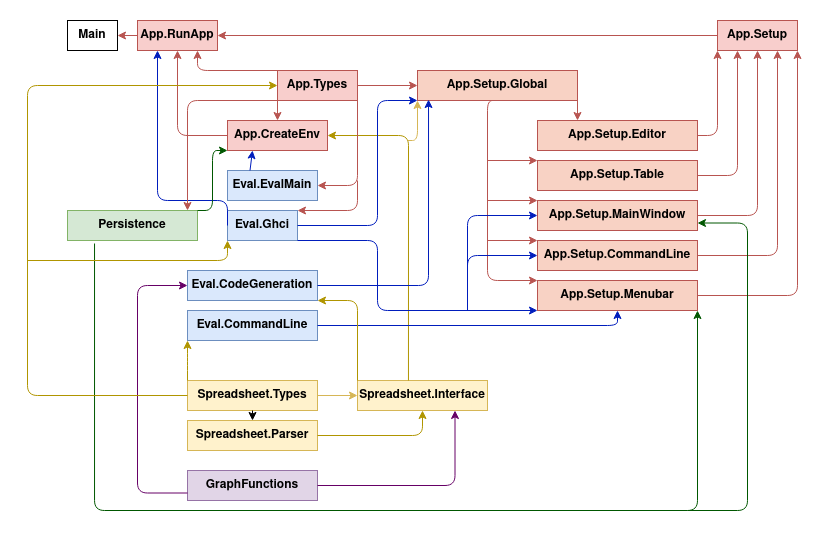
\includegraphics[width=\textwidth]{ApplicationStructure}
	\caption{A modulok közti függőségek}
	\label{fig:appstructure}
\end{figure}

\section{GraphFunctions}

\begin{figure}[H]
	\centering
	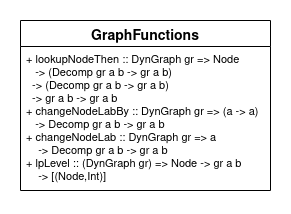
\includegraphics[width=\textwidth]{GraphFunctions}
	\caption{A Graphfunctions komponens interfésze}
	\label{fig:appstructure}
\end{figure}
\section{Spreadsheet}

\subsection{Áttekintés}

\begin{figure}[H]
	\centering
	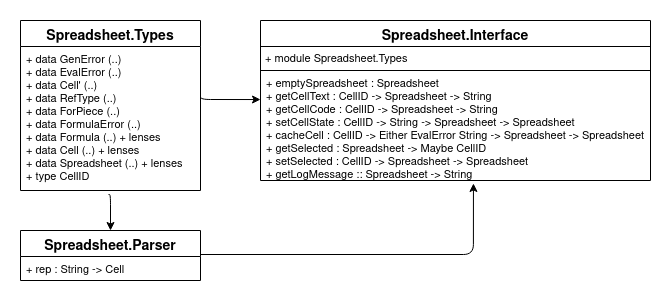
\includegraphics[width=\textwidth]{Spreadsheet}
	\caption{A Spreadsheet komponens moduljainak kapcsolata és interfésze}
	\label{fig:appstructure}
\end{figure}

\subsection{Spreadsheet.Types}

Az alkalmazás a Spreadsheet típussal reprezentálja a számolótábla állapotát. Alább látható a Spreadsheet.Types modulban szereplő definíció:

\lstset{caption={A Spreadsheet típus}, label=src:hs2}
\begin{lstlisting}[language={Haskell}]
type CellID = Int

data Cell' = Str String | Number Double | EmptyCell

data RefType = Absolute | Relative

data ForPiece = Code String | Refs [(CellID, RefType, RefType)]

data FormulaError = FNoParse
                  | FCycleRefError
                  | FNoCache
                  | FListTypeError
                  | FMissingDepError
                  | FGhciError
                  | FTimeoutError

data Formula = Formula { _code :: String
                       , _cache :: Either FormulaError Cell'
                       , _value :: Maybe [ForPiece]
                       }

data Cell = Val {_cellV :: Cell'} | For {_cellF :: Formula}

data Spreadsheet = SS { _sheet :: Gr Cell Int
                      , _selected :: Maybe CellID
                      , _logMessage :: Maybe String
                      }
\end{lstlisting}

A Spreadsheet egy rekord típus, melynek három mezője van. A \textit{\_selected} mező jelenti az aktuálisan kijelölt cellát. Ez a mező kerülhetett volna a globális állapotba is, azonban a tervezés korai fázisában más döntés született, és a későbbiekben körülményes lett volna refaktorálni a kódot. (Ugyanakkor ennek átírása tervben van az alkalmazás egy későbbi verziójában.) A \textit{\_logMessage} mező tartalmazza a legutóbbi művelet kiértékeléséből származó szöveges (a GUI-ban a logra írandó) üzenetet.

A \textit{\_sheet} mező reprezentálja a tényleges számolótáblát. A számolótábla egy irányított gráf, aminek a csúcsai \textit{Cell} típusú értékekkel vannak címkézve. Az élek egész számokkal vannak címkézve. (A számszerű élcímkékre csak a használt gráfcsomag által biztosított útkereső algoritmus megszorításai miatt van szükség. Az alkalmazás implementációjában minden él címkéje \textit{1}.) A gráfban minden csúcs a számolótábla egy cellájának felel meg. Egy \textit{A} csúcsból pontosan akkor megy él egy \textit{B} csúcsba, ha a \textit{B} csúcsban található cella kódja hivatkozik az \textit{A} csúcsban található cellára. 

Egy cella pontosan akkor szerepel a gráfban, ha nemüres vagy van olyan cella, amelyik hivatkozik rá. Így az egyszerre üres és nemhivatkozott cellák tárolására nincs szükség.

A fent megadott gráfreprezentációnak két további előnye is van. Egyrészt könnyű körfigyelést implementálni, így elkerülve, hogy cellák körkörösen hivatkozzanak egymásra; másrészt ha módosul egy \textit{A} cella tartalma, akkor pontosan az \textit{A}-ból elérhető csúcsoknak megfelelő cellákat kell újra kiértékelni.

A gráfreprezentáció megvalósításához az \textit{fgl} csomagot használtam. A \textit{Spreadsheet} típus definíciójában a PatriciaTree alapú \textit{Gr} típust használtam. A műveletek a \textit{DynGraph} típusosztály tetszőleges megvalósítására működnek, így lehetséges a belső gráfreprezentáció cseréje tetszőleges másik, \textit{DynGraph} példánnyal rendelkező típusra.

Egy cella tartalmát a \textit{Cell} típus reprezentálja. Egy cella tartalma lehet érték (\textit{Cell'}) vagy formula (\textit{Formula}). Az érték jelenleg háromféle lehet: szám (\textit{Double}), string vagy üres.

Ha egy cella formulát tartalmaz, az a háromelemű \textit{Formula} rekorddal reprezentáltatik. A \textit{\_code} mező tartalmazza a felhasználó által megadott kódot. Ez egy kényelmi funkció, hogy a kód megjelenítéséhez ne kelljen visszakonvertálni a reprezentációból. A \textit{\_cache} mezőben szerepel, hogy mi a formula legutóbbi kiértékelésének eredménye (ha egyáltalán már ki lett értékelve). A cache értéke vagy egy érték (\textit{Cell'}) vagy valamilyen hiba (\textit{FormulaError}). 

A \textit{\_value} jelenti a formula kódgeneráláshoz szükséges reprezentációját.  Ez a reprezentáció \textit{ForPiece}-ek (formuladarabok) listája. Egy formuladarab vagy egy kódrészlet (\textit{String}) vagy cellaazonosítók listája, jelölve rendre azt is, hogy a hivatkozás abszolút vagy relatív az oszlopra és sorra nézve (\textit{RefType}). A hivatkozás típusának (relatív/abszolút) csak másoláskor és mozgatáskor van jelentősége. Jelenleg ezen funkciókhoz nincsenek is használva a \textit{\_value} mezőben tárolt \textit{RefType}-ok, de a szoftver további fejlődési lehetőségeire gondolva szerepelnek a reprezentációban.

A \textit{\_value} mezőről részletesebben lesz szó a \textit{Spreadsheet.Parser} és a \textit{Spreadsheet.CodeGeneration} modulok leírásában. 

A \textit{Formula} típushoz tartozik egy invariáns állítás: a program futása során egy \textit{Formula} mindig a 3.1 táblázatban leírt állapotok valamelyikében figyelhető meg.

\begin{table}
	\centering
	\begin{tabularx}{\textwidth}{ |l l l l| X |}
		\hline
		\multicolumn{4}{|c|}{Minta} & \multicolumn{1}{|c|}{Jelentés} \\
		\hline\hline
		Formula & \_ & (Left FNoParse) & Nothing & parseolási hiba \\
		\hline
		Formula & \_ & (Left FCycleRefError) & Nothing & sikeres parseolás, azonban a formula körkörös referenciákat adott volna a táblához \\
		\hline
		Formula & \_ & (Left FNoCache) & (Just \_) & sikeres parseolás, érvényes referenciák, de a formula még nem lett kiértékelve \\
		\hline
		Formula & \_ & (Left FListTypeError) & (Just \_) & \textbf{\textit{nem használt}} \\
		\hline
		Formula & \_ & (Left FMissingDepError) & (Just \_) & a formula nem értékelhető ki, mivel egy hivatkozott cella nem volt cache-elve. \\
		\hline
		Formula & \_ & (Left FGHCIError) & (Just \_) & a formula egyéb okokból nem volt kiértékelhető (pl. típushiba, Haskell szintaxishiba) \\
		\hline
		Formula & \_ & (Left FTimeoutError) & (Just \_) & időtúllépés miatt sikertelen kiértékelés, valószínűleg végtelen ciklus miatt \\
		\hline
		Formula & \_ & (Right cell') & (Just \_) & sikeres kiértékelés, az eredmény cell' \\
		\hline 
	\end{tabularx}
	\caption[Egy \textit{Formula} lehetséges állapotai]{Egy \textit{Formula} lehetséges állapotai}
	\label{tab:formula}
\end{table}

Érdemes megjegyezni, hogy ez az invariáns típuszinten is garantálható lett volna (feladat az olvasó számára!). A jelenlegi megoldás a korai tervezési fázis eredménye, a későbbiekben már erőforrásigényes lett volna refaktorálni a kódot.   

További megjegyzések a \textit{Spreadsheet} típussal kapcsolatban:
\begin{compactenum}
	\item A \textit{Spreadsheet.Types} modul alapértelmezett nevű lenseket is exportál a \textit{Cell, Formula} és \textit{Spreadsheet} típusokhoz.
	\item A \textit{Spreadsheet.Types} modulban szereplő összes típus (a kivételek kivételével) példánya a \textit{Generic} és \textit{Serialize} típusosztályoknak (ez utóbbit a \textit{cereal} csomag exportálja). Erre a perzisztencia implementációjához van szükség.
	\item A \textit{FormulaError} típus \textit{FListTypeError} konstruktora jelenleg nincs használva. Ez a konstruktor azt jelezné, ha egy hivatkozáslista nem értelmes, mert a hivatkozott cellák listája nem homogén. Ez jelenleg nem ellenőriztetik, az inhomogén listák által okozott hibák csak a kiértékelés során jelentkeznek. Amennyiben a későbbiekben implementálásra kerülne ez a funkció, lehetséges az \textit{FListTypeError} konstruktor felhasználása.
\end{compactenum} 

\subsection{Spreadsheet.Parser}

A modul feladata egy a felhasználó által egy cellához megadott kód (\textit{String}) reprezentációjának (\textit{Cell}) előállítása. A modul egy függvényt exportál: \mbox{(\textit{rep :: String -> Cell)}}

Legyen a felhasználó által megadott kód \textit{str}. A \textit{rep} függvény az alább leírt specifikáció szerint állítja elő a kód cellareprezentációját. A reguláris kifejezések megadásakor a kifejezésre illeszkedő string előtt és után tetszőlegesen sok szóköz lehet, ha nincs másképp jelezve.

\begin{compactenum}
	\item Ha str = "", rep str = \textit{Val EmptyCell}
	\item Ha str illeszkedik a $((+|-|\varepsilon)D^+(.D^*|\varepsilon))|.D^+)$ reguláris kifejezésre, ahol D=(0|1|2|3|4|5|6|7|8|9), akkor rep str = \textit{Val (Num n)}, ahol \textit{n} a literál által ábrázolt lebegőpontos szám. 
	\item Ha a fenti esetek egyike sem áll fent, és str nem (=C*) alakú (ahol C az összes karakterek halmaza), akkor rep str = \textit{Val (Str str)}
	\item Ha B a betűk halmaza (a \textit{Data.Char} modul \textit{isLetter} függvényének igazsághalmaza), C' = $C \backslash \{\S\}$ és str \mbox{$(=((\S  (\varepsilon|\$)B(\varepsilon|\$)D^+:(\varepsilon|\$)B(\varepsilon|\$)D^+\S )|(\S (\varepsilon|\$)B(\varepsilon|\$)D^+\S )|(C'^+))^+)$} alakú, akkor a kód formulaként parseolható. rep str = \textit{Formula str (Left FNoCache) (Just ps)}, ahol ps definíciója alább szerepel.
	\item Ha egyik fenti eset sem áll fent, akkor a parseolás sikertelen. Ekkor rep str = \textit{Formula str (Left FNoParse) Nothing}
\end{compactenum}

Ha \textit{str} formulaként parseolható (fenti 4. eset), egy egyszerű szintaktikus elemzés segítségével kaphatjuk a reprezentációjának \textit{\_value} komponensét. A parser először elhagyja az \textit{=} karaktert. Ezután sorban parseol substringeket a szó elejéről az alábbi módon:
\begin{compactenum}
	\item Először megpróbálja cellahivatkozásként olvasni a soron következő részt: $((\S  (\varepsilon|\$)B(\varepsilon|\$)D^+:(\varepsilon|\$)B(\varepsilon|\$)D^+\S )|(\S (\varepsilon|\$)B(\varepsilon|\$)D^+\S ))$. Ha sikerült, a hivatkozást cellaazonosítók sorozatává konvertálja (lásd alább), és a kapott \textit{rs} azonosítólistát $Refs\ rs$ módon az eredménylista végére fűzi.
	\item Ha a soron következő substring nem olvasható cellahivatkozásként, akkor a parser végigolvassa a lehető leghosszabb $s = C'^+$ substringet, és az eredménylistához egy $Code\ s$-t ír.
\end{compactenum}

A cellahivatkozások feloldásához kihasználjuk, hogy a karakterek injektíven az egész számok halmazára képezhetők (az \textit{Enum} típusosztály műveleteivel). A kis- és nagybetűket nem különbözetjük meg. Emellett felhasználjuk az \textit{(Int,Int)} párokra definiált \textit{Enum} példányt is. (lásd 3.2.4) Ez a példány csak nemnegatív elemű párokra működik helyesen, de a program számára ez is elég. Jelölje $fromEnum^C$ a karaktert Int-té kódoló függvényt, és $fromEnum^P$ az \textit{(Int,Int)} párt Int-té kódoló függvényt. Jelölje $a,b :: Int$ esetén $[a..b]$ az $a \le n \le b$ n egész számok rendezett listáját! Ekkor a cellahivatkozások feloldása az alábbiak szerint történik:
\begin{compactenum}
	\item Ha a hivatkozás $(\S (\varepsilon|\$)B(\varepsilon|\$)D^+\S )$ alakú, legyen \textit{b} a betű, és \textit{n} a számjegyek által reprezentált egész szám. Ekkor a kapott  \textit{rs} lista egyelemű. $rs\ = [(fromEnum^P\ (fromEnum^C,n), rt1, rt2)]$ Itt $rt1,rt2 :: RefType$. Ha az oszlopnév előtt volt \$, $rt1=Absolute$, különben $rt1=Relative$. Ha a sornév előtt volt \$, $rt2=Absolute$, különben $rt2=Relative$.
	\item Ha a hivatkozás $(\S  (\varepsilon|\$)B(\varepsilon|\$)D^+:(\varepsilon|\$)B(\varepsilon|\$)D^+\S )$ alakú, felbontható a \textit{:} mentén két egyszerű hivatkozásra. Legyenek a betűk $d_1$ és $d_2$, a számjegyek által reprezentált számok pedig rendre $n_1$ és $n_2$! Ekkor haskelles listakifejezésként a következő módon definiálhatjuk a kapott azonosítólistát: $rs =$ \mbox{$[(fromEnum^P (r,c), rt1, rt2) | r \leftarrow [fromEnum^C(d_1)..fromEnum^C(d_2)], c \leftarrow [n_1..n_2]]$} $rt1$ és $rt2$ az előző esethez hasonlóan kerül meghatározásra, de a $:$ előtti referenciában található $\$$ alapján dől el, hogy az oszlop és a sor abszolút vagy relatív.
	
\end{compactenum}

\subsection{Spreadsheet.Interface}

Ebben a modulban szerepelnek az \textit{App} komponens számára elérhető, a \textit{Spreadsheet} típushoz kapcsolódó függvények. A 3.2 táblázatban szerepel a modul által exportált függvények feladatainak listája.

\begin{table}
	\centering
	\begin{tabularx}{\textwidth}{ |l|X|X|}
		\hline
		Függvény  & Feladat \\
		\hline\hline
		emptySpreadsheet &  üres számolótábla (0 csúcsú gráf, nincs kijelölt cella, nincs log üzenet) \\
		\hline
		getCellText & egy cellában megjelenítendő szöveg lekérdezése \\
		\hline
		getCellCode & egy adott cellába legutóbb beírt kód lekérdezése \\
		\hline
		setCellState & a megadott cella állapotának módosítása egy a felhasználó által megadott String alapján \\
		\hline
		cacheCell & kiértékelés eredményének cachelése \\
		\hline
		getSelected & kijelölt cella azonosítója \\
		\hline
		setSelected & kijelölt cella azonosítójának beállítása \\
		\hline 
		getLogMessage & legutóbbi log üzenet lekérdezése \\
		\hline
	\end{tabularx}
	\caption[A \textit{Spreadsheet.Interface} által exportált függvények]{A \textit{Spreadsheet.Interface} által exportált függvények}
	\label{tab:interface}
\end{table}

\subsubsection{setCellState :: CellID -> String -> Spreadsheet -> Spreadsheet}

A \textit{setCellState} függvény feladata, hogy a megadott cellaazonosítóhoz tartozó csúcsban lévő cella állapotát a felhasználó által megadott \textit{String}-nek megfelelően módosítsa, valamint felülírja a \textit{\_logMessage} mező tartalmát a múvelet sikerességétől függően.

Ehhez szükség van a megadott \textit{String} \textit{Cell} reprezentációjára, amit a \textit{Spreadsheet.Parser} modul által exportált \textit{rep} függvény számít ki. A kapott reprezentáció alapján az alább leírtaknak megfelelően viselkedik a függvény:

\begin{compactenum}
	\item Ellenőrzi, hogy a cella állapotának megváltoztatásával keletkeznék-e 		körkörös referencia. Pontosan akkor keletkeznék, ha a megváltoztatandó $c$ 	azonosítójú cellához tartozó csúcsba bemenő összes él kitörlésével keletkezett gráfban van olyan $n$ azonosítójú csúcs, hogy $c$ kódja hivatkozik $n$-re és a gráfban már van $c \rightarrow n$ út. (Ez utóbbi feltétel azt jelenti, hogy az $n$ cella értéke függ $c$ értékétől.) Ezt a feltételt az \textit{isLegal} segédfüggvény ellenőrzi. Érdemes megjegyezni, hogy ilyen hiba csak akkor fordulhat elő, ha a kapott reprezentációnk egy formula.
	\item Amennyiben az \textit{isLegal} eredménye \textit{False}, a $c$ csúcsban levő cella reprezentációja \textit{For (Formula str' (Left FCycleRefError) Nothing)} lesz, ahol \textit{str'} a paraméterként kapott \textit{String}. A \textit{\_logMessage} mezőbe egy hibaüzenet kerül.
	\item Amennyiben az \textit{isLegal} segédfüggvény \textit{True} eredményt ad, a gráfból kitöröltetik az összes $c$-be menő él, és új $c$-be menő élek kerülnek behúzásra a $c$ kódja által referált celláknak megfelelő csúcsokból. (Ezeket a \textit{references} segédfüggvény számolja a reprezentációból.) A \textit{\_logMessage} mező tartalma egy sikert jelző üzenet lesz.
	\item Amennyiben a módosított cella üressé vált, az összes olyan üres cellához tartozó csúcs kitöröltetik a gráfból, melyekből csak a módosított cellába ment él.
	\item Amennyiben a módosított cella üressé vált, és a hozzátartozó csúcs kifoka 0 (nem hivatkozik más cella az üressé tett cellára), úgy a csúcs töröltetik a gráfból.
\end{compactenum}

Megjegyzés: az utolsó két pont garantálja, hogy nem a program nem tárol feleslegesen cellákat a gráfban.

\subsubsection{cacheCell :: CellID -> Either EvalError String -> Spreadsheet -> Spreadsheet}

A függvény feladata, hogy a megadott cellaazonosítóhoz tartozó csúcsban lévő cella állapotát frissítse a kiértékelés során kapott eredménnyel. A frissítendő cella szükségszerűen egy formula, a \textit{cacheCell} ennek \textit{\_cache} mezőjét módosítja az alábbiak szerint:

\begin{compactenum}
	\item Ha a kiértékelés eredménye hiba (a második paraméter \textit{Left}), akkor a cache-be a megfelelő hiba kerül.
	\item Ha a kiértékelés eredménye értelmes (a második paraméter \textit{Right}), akkor a függvény értékként parseolja a kapott eredményt, és a parseolt értéket írja a cache-be.
\end{compactenum}

\section{Eval}

\subsection{Áttekintés}

\begin{figure}[H]
	\centering
	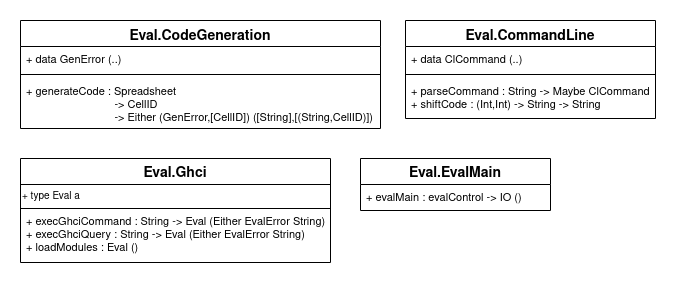
\includegraphics[width=\textwidth]{Eval}
	\caption{Az \textit{Eval} komponens moduljainak kapcsolata és interfésze}
	\label{fig:appstructure}
\end{figure}

\subsection{Eval.CodeGeneration}

A kiértékelési folyamat az alábbi szempontok alapján került megtervezésre:
\begin{compactenum}
	\item Listán értelmezett függvények esetén legyen lehetőség könnyen kezelni az üres cellákat, alapértelmezett értékek megadásával.
	\item Ha a kiértékelés során hiba történik, annak hatása minimális legyen.
\end{compactenum}

Az első szempont megvalósításához a kiértékelés során egy kiszámított vagy paraméterként kapott \textit{a} típusú értéket egy \textit{Maybe a} típusú érték reprezentálja. Az üres cellákat \textit{Nothing} reprezentálja, az értékkel rendelkező cellákat pedig egy \textit{Just} érték. Egy a kiértékelés során kiszámított cellaérték is mindig egy \textit{Just}-ba csomagoltatik. Ennek megfelelően \textit{a} típusú cellaértékek listájának futásidejű reprezentációja egy \textit{[Maybe a]}. A Haskellben megszokott listafüggvények a felhasználói dokumentációban részletesen leírt függvények segítségével használhatók ezen a reprezentáción.

A második szempont megvalósításához a kódgenerálás során értékadások sorozata jön létre, és a kiértékelés során ezen értékadások egyesével hajtódnak végre. Így ha valamelyik cella kiértékelésének eredménye egy hiba, csak a tőle függő cellák értéke lesz hiba. 

Ha sikeres a generálás, a \textit{generateCode} függvény eredménye két (egy \textit{Right} konstruktorba csomagolt) lista (\textit{[String],[(String,CellID)]}. Az első listába kerülnek az értékadások, amelyek az úgynevezett külső függőségekhez lettek generálva. A második lista tartalmazza az olyan értékadásokat, amelyek a megváltoztatott id-jű cellától függnek. A \textit{Spreadsheet.Types} modulnál tárgyalt gráfreprezentáció segítségével az előbbi két fogalmat az alábbi módon tehetjük precízzé: 

Legyen \textit{id} a megváltoztatott cella azonosítója, és legyen $lab : CellID \rightarrow Cell$ a gráf csúcsaihoz a megfelelő cellát hozzárendelő függvény! Legyenek $For,Lab : Cell \rightarrow \mathbb{L}$ predikátumok, amelyek akkor adnak igazat, ha a paraméterük a megfelelő konstruktorral jött létre. Legyen \textit{b} egy létező cellaazonosító! Ekkor:
\begin{align*}
	\text{b külső függőség} &\Leftrightarrow \exists c: (\exists (id \rightarrow c \text{ út}) \wedge \exists (b \rightarrow c \text{ út}) \wedge \not\exists  (id \rightarrow b \text{ út})) \\
	& \vee((b=id) \wedge Val(lab(b))) \\
	\text{b függ id-től} &\Leftrightarrow ((b \not= id) \wedge \exists (id \rightarrow b \text{ út}) \\
	&\vee ((b = id) \wedge For(lab(b)))
\end{align*}

Az \textit{id}-től függő olyan módon kell sorrendbe rendezni, hogy az eredménylistában egy cella csak az őt a listában megelőző celláktól függjön. Ekkor az értékadásokat lehetséges a lista által megadott sorrendben kiértékelni. A sorba rendezéshez a leghosszabb utak algoritmusa szerinti szintek használatosak, ezek alapján kerülnek növekvő sorrendbe az \textit{id}-től függő cellák. Könnyű látni, hogy ez a sorrend megfelel a fent megfogalmazott elvárásnak.  

A kódgeneráláshoz szükséges ellenőrizni, hogy a kapott külső függőségek értéke kiolvasható-e. Ez akkor lehetséges, ha a külső függőség egy \textit{Val} (de nem \textit{Val EmptyCell}), vagy egy olyan \textit{For}, amelybe van cachelve érték.

Az \textit{id}-től függő cellák esetén (ezek szükségszerűen formulák) azt kell ellenőrizni, hogy sikerült-e őket parseolni. Ez ekvivalens azzal, hogy a \textit{\_value} mező értéke \textit{Just}.

A függőségek listáinak kiszámítása és a fenti ellenőrzések elvégzése a \textit{depList} függvény feladata. A leghosszabb utak szerinti szinteket kiszámító függvény a \textit{GraphFunctions} modulban szerepel. 

Az értékadások generálásáért a \textit{codeG} függvény felel. Ez az \textit{n} azonosító cellához egy \textit{vn = someCode} formájú értékadást generál. A \textit{someCode} részt külső függőség esetén a \textit{cacheG}, \textit{id}-től függő cella esetén a \textit{cellG} függvény számítja ki.

A \textit{cacheG} függvény üres cellákhoz a \textit{"Nothing"} stringet rendeli. Számokhoz és stringekhez pedig egy \textit{"Just val"} stringet, ahol \textit{val} a megfelelő szám/string. Amennyiben egész számról van szó, a függvény levágja a tizedesrészt a számliterálról, hogy a GHCi egész típusúként értelmezhesse a literált.

A \textit{cellG} függvény a formula \textit{\_value} komponensének elemeiből egy stringet állít elő. Ehhez a \textit{\_value} mező minden eleméhez egy stringet rendel, és ezeket konkatenálja, majd a legvégén eléír egy \textit{"Just \$ "}-t. A függvény az egyes elemekhez az alábbi módon rendel stringeket:
\begin{compactenum}
	\item \textit{Code code} $\rightarrow$ code
	\item \textit{Refs [n]} $\rightarrow$ "fromJust v\textit{n}"
	\item \textit{Refs ids}, ha $|ids| > 1 \ \rightarrow$ az ids-ben szereplő cellaazonosítókból generált változónevek listája. Pl. ids=\textit{[1,2,3]} esetén \textit{"[v1,v2,v3]"}
\end{compactenum}

A fenti leírásból jól látszik, hogy egy cella értéke mindig \textit{Just}-ba lesz csomagolva. Ha egy cella értékét akarjuk használni, az a "szokásos módon" megtehető, mivel a változónév elé egy \textit{fromJust} kerül. Cellák listája esetén azonban \textit{Just} értékek listáját kapjuk. Érdemes megjegyezni, hogy a cellákhoz kiszámított érték mindig \textit{Maybe a} típusú lesz, így az eredmény kinyeréséhez a \textit{fromJust vn} kód szükséges. Ha az eredmény \textit{Nothing}, ez futásidejű hibát okoz, amit a hívó ki tud olvasni a GHCi-ból, és cachelhet egy hibát a kiértékelt cellához (\textit{EGhciError}). Ez a viselkedés az \textit{App.Setup.Global.evalAndSet} függvényben van definiálva.

A modul által exportált \textit{generateCode} függvény segítségével végezhető el a fent leírt kódgenerálás. 

\subsection{Eval.EvalMain}

A modul által exportált \textit{evalMain} függvény a kifejezések GHCi-ben való kiértékelését végző szál főprogramja. A szál az alábbiak szerint működik:

\begin{compactenum}
	\item Várakozik, ameddig a globális állapot \textit{evalControl} mezőjének \textit{eCommand} változójába egy GHCi utasítást nem ír a fő szál.
	\item Kiüríti a változót, és kiértékeli a kapott utasítást a GHCi-ben.
	\item Ha egy megadott idő után nem ér véget a kiértékelés (jelenleg 1 másodperc), lekérdezi a GHCi folyamathoz tartozó PID-et, majd megkeresi annak a gyerekfolyamatát (\textit{childPid}), és az \textit{eResult} változóba \textit{Left\ childPid}-et ír. Ezt a folyamatot aztán a fő szál fogja kilőni.
	\item Amennyiben időben véget ér a kiértékelés, a GHCi által eredményül adott sorok \textit{result} listáját \textit{Right\ result} módon az \textit{eResult} változóba írja.
\end{compactenum}

Az időtúllépés utáni viselkedés bonyolultsága egy szerencsétlen helyzet eredménye. A magyarázathoz meg kell ismerni a \textit{ghcid} csomag által biztosított GHCi interfészt. A \textit{startGhci} függvény a dokumentáció alapján elindít egy GHCi háttérfolyamatot, amellyel innentől egy megadott szálról kell interaktálni (a megszakítást kivéve). A valóságban azonban azt tapasztaltam, hogy két folyamatot indít el, amelyek közül az egyik gyereke a másiknak. 

Időtúllépés esetén meg kell állítani a háttérben futó számítást. Erre szolgálna az \textit{interrupt} függvény, ami egy \textit{SIGINT} jelzést küld a GHCi folyamatnak. A GHCi folyamat azonban bizonyos esetekben ezt kimaszkolja, ilyenkor a számítást nem lehetséges az \textit{interrupt} segítségével megszakítani. A GHCi leállítására szolgáló \textit{stopGhci} függvény pedig csak  az egyik (a szülő) folyamatot terminálja a \textit{startGhci} által indított két folyamatból. A másik folyamat pedig tovább folytatja a számítást. Az alkalmazás egy Haskell szálat tartalmazó verziójában ez kiéheztette a fő folyamatot. 

Ezért van szükség arra, hogy a kiértékelés külön szálon fusson. Ugyanis időtúllépés esetén a fő szál, miután ütemezésre kerül, a kapott PID alapján a lehető legagresszívabban (\textit{SIGKILL}) terminálja a második GHCi folyamatot. Ez a tapasztalat szerint az első folyamatnak is véget vet, és semmilyen erőforrást nem szivárogtat. A folyamat terminálása után új GHCi folyamat indítható.

A fenti megoldást a szükség szülte, és tapasztalatok alapján, próbálgatás útján állt össze. Nem ismert, hogy miért indít a \textit{startGhci} két folyamatot. (Egy konzolból indított GHCi folyamathoz például csak egy PID tartozik.) A megoldás az én számítógépemen, Ubuntu 20.04 LTS operációs rendszer mellett működött, de nincs rá garancia, hogy más Linux rendszer (vagy akár egy másik számítógép!) esetén működni fog. (A működés feltétele, hogy ütemezésre kerüljön a fő szál.) Ráadásul csak e miatt az interakció miatt kellett konkurrenciát adni az alkalmazáshoz. Valódi hatékonyságot ezzel nem nyertünk, hiszen az egyik szál mindig blokkolt állapotban lesz. (Mivel mindkét szál a fogyasztóként hozzá tartozó \textit{MVar}-ra várakozik, ha éppen a másik szál dolgozik.)

A gyerekfolyamat megtalálásához a program rendszerhívást hajt végre, a \textit{pgrep} parancsot használja \textit{-P} kapcsolóval.

Megjegyzés: a fent leírt információk két StackOverflow diskurzusból \cite{ghci_stackoverflow1} \cite{ghci_stackoverflow2} származnak. Ezekben további hivatkozások is elérhetők, melyek segítenek megérteni a problémát.

\subsection{Eval.Ghci}

A modul fő feladata, hogy kiértékeljen egy GHCi parancsot, és az eredményt értelmezze. Emellett lehetőséget biztosít a modulok és keresési útvonalak újratöltésére a globális konfiguráció alapján (\textit{EvalConfig}).

A kiértékelés folyamata a (nem exportált) \textit{execG} függvényben van leírva, és az alábbi módon zajlik:
\begin{compactenum}
	\item A paraméterként kapott parancs a \textit{eCommand} változóba kerül.
	\item Kiolvasásra kerül az eredmény az \textit{eResult} változóból.
	\item Ha az eredmény \textit{Left\ pid}, a kapott PID-hez tartozó folyamat terminálásra kerül, és a kiértékelés eredménye \textit{Left\ ETimeoutError}. Új GHCi folyamat indul, és a hivatkozása bekerül a globális állapot \textit{evalConfig} mezőjének \textit{eGhci} mezőjébe.
	\item Ha az eredmény \textit{Right\ result}, ez a kiértékelés eredménye. \textit{result :: [String]} a GHCi által eredményül adott sorok listája.
\end{compactenum}

Az exportált \textit{execGhciCommand} függvény ezt a viselkedést egészíti ki egy extra ellenőrzéssel.
\begin{compactenum}
	\item Ha az \textit{execG} eredménye \textit{Left\ ETimeoutError}, akkor ez az eredmény.
	\item Ha az \textit{execG} eredménye \textit{Right\ results}:
	\begin{itemize}
		\item Ha \textit{results} üres, az eredmény \textit{Right\ ""}
		\item Ha \textit{results} egyelemű, az eredmény \textit{Right\ (head (results))}
		\item Ha \textit{results} több elemű, akkor a GHCi több sornyi eredményt adott vissza. Ezt a függvény hibának tekinti, és az eredmény \textit{Left (EGhciError results)}
	\end{itemize}
\end{compactenum}

A \textit{loadModules} akció beállítja a globális állapot \textit{evalControl} mezőjének \textit{eConfig} mezője alapján az elérési utakat, majd betölti a megadott modulokat. A korábban betöltött modulokat először kitölti (\textit{:m}). Ilyenkor a felhasználó által közvetlenül a GHCi-ba megadott definíciók is elvesznek. Az akció betölti az \textit{Empty} modult is (standard könyvtár).

\subsection{Eval.CommandLine}

A modul feladata a felhasználó által a parancssorba beütött parancsok reprezentációjának előállítása, amely alapján a parancsok végrehajthatók. A parancsok reprezentációját a \textit{ClCommand} típus adja:

\lstset{caption={A \textit{ClCommand} típus}, label=src:clcommand}
\begin{lstlisting}[language={Haskell}]
data ClCommand = ClGhci String
               | ClMv ((Int,Int),[(CellID, CellID)])
               | ClCp ((Int,Int),[(CellID, CellID)])
\end{lstlisting}

A \textit{ClGhci} konstruktorral létrehozott parancs a GHCi-ban értékelendő ki. A másik két konstruktor az \textit{mv} és \textit{cp} parancsokhoz szolgál. Ezen konstruktorok második paramétere a forrás-cél cellaazonosító-párok listája, az első paraméter pedig ezen azonosítópárok koordinátánkénti távolsága. A parancsok parseolása megfelel a felhasználói dokumentációban leírtaknak. A referenciák feloldása a \textit{Spreadsheet.Parser} dokumentációjában leírtak szerint történik.

A modul exportálja a \textit{parseCommand :: String -> Maybe ClCommand} függvényt, amely a fent leírtaknak megfelelően elvégzi a parseolást. Hiba esetén az eredmény \textit{Nothing}, sikeres parseolás esetén pedig \textit{Just}.

A modul emellett exportálja a \mbox{\textit{shiftCode :: (Int,Int) -> String -> String}} függvényt, amely egy cella (feltételezetten helyesen parseolható) kódját (\textit{String} paraméter) "eltolja" az \textit{(Int,Int)} paraméter által megadott vektorral (oszlop eltolás, sor eltolás). Ez azt jelenti, hogy az összes relatív hivatkozást módosítja, az abszolút hivatkozásokat azonban helybenhagyja.

\section{Persistence}

\begin{figure}[H]
	\centering
	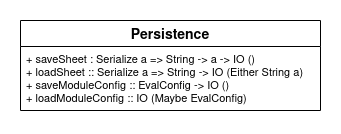
\includegraphics[width=\textwidth]{Persistence}
	\caption{Az \textit{Persistence} komponens interfésze}
	\label{fig:appstructure}
\end{figure}


A modul feladata, hogy fájlokat mentsen és betöltsön. Egy adatot akkor lehet elmenteni, ha az adat típusa példánya a \textit{Serialize} típusosztálynak. Ezt a típusosztályt a \textit{cereal} csomag biztosítja. Egy \textit{Serialize} példány minden eleme bytestring-gé szerializálható. A program a számolótáblák és a konfigurációs fájlok perzisztálásához is bytestring formátumot használ.

Jelenleg a program egy konfigurációs fájlt használ, ennek nevét a \textit{moduleConfigFile} konstans definiálja. Az alkalmazás bezárásakor ebbe a fájlba kerül mentésre a globális állapot \textit{evalControl} mezőjének \textit{eConfig} mezője.

\subsubsection{saveSheet :: Serialize a => String -> a -> IO ()}

Ez a függvény elment egy szerializálható adatot a megadott fájlnévvel. Létező fájl esetén felülírás történik. 

\subsubsection{loadSheet :: Serialize a => String -> IO (Either String a)}

Betölti a paraméterként kapott fájlból az adatot. Ha nem létezik a fájl, az eredmény egy hibaüzenet, ami jelzi, hogy a paraméterként kapott fájl nem létezik.

\subsubsection{saveModuleConfig :: EvalConfig -> IO ()}

A \textit{saveSheet} speciális esete. A kapott paramétert a \textit{moduleConfigFile} konstans által megadott fájlba menti.

\subsubsection{loadModuleConfig :: IO (Maybe EvalConfig)}

Betölti a modulkonfigurációs fájl tartalmát. Ha a fájl nem létezik, az akció eredménye \textit{Nothing}.

\section{App}

\subsection{Áttekintés}

\begin{figure}[H]
	\centering
	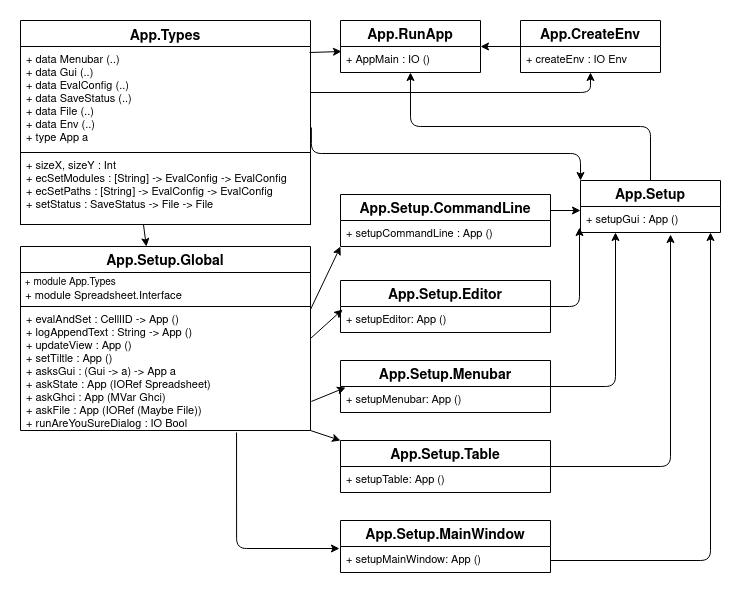
\includegraphics[width=\textwidth]{App}
	\caption{Az \textit{App} komponens moduljainak kapcsolata és interfésze}
	\label{fig:appstructure}
\end{figure}

\subsection{App.RunApp}

Ez a modul definiálja a főprogramot (\textit{appMain :: IO () )}, amellyel egyenlő a \textit{Main}-ben definiált \textit{main} függvény. Az \textit{appMain} két akcióból áll. Először inicializálja az olvasható globális állapotot (\textit{App.CreateEnv.createEnv}), majd végrehajtja a \mbox{\textit{runApp :: ReaderT Env IO ()}} akciót, az olvasható globális állapotot az előbb inicializált környezetre állítva. A 
\textit{createEnv} akció elindítja a háttérben futó kiértekelő szálat is. (\textit{Eval.EvalMain.evalMain}).

A \textit{runApp} akció a következőképpen határozza meg a program működését:
\begin{compactenum}
	\item Hozzárendeli a GUI elemeihez az eseménykezelőket (\textit{App.Setup.setupGui}).
	\item Betölti a beállított keresési útvonalakat és modulokat a GHCi-be (\textit{Eval.Ghci.loadModules}). Ha nem található a konfigurációs fájl, egy figyelmeztetést ír a standard kimenetre.
	\item Beállítja, hogy az alkalmazás bezárásakor álljon le a GHCi és a modulok konfigurációja kerüljön mentésre.
	\item Megjeleníti a GUI-t és elindítja a main loopot. 
\end{compactenum}

\subsection{App.CreateEnv}

Ez a modul exportálja az \textit{App.RunApp}-ban használt \mbox{\textit{createEnv :: IO Env}} akciót.

A \textit{createEvalControl :: IO EvalControl} segédakció hozza létre az \textit{evalControl} mező tartalmát. Az \textit{eGhci} mezőhöz elindít egy GHCi-t. A GHCi alapértelmezett munkakönyvtára az alkalmazás futtatásának helye. Az \textit{eCommand} és \textit{eResult} mezőkhöz létrehoz egy-egy üres \textit{MVar}-t. Az \textit{eConfig} mező tartalmát beolvassa a konfigurációs fájlból (\textit{Persistence.loadModuleConfig}).

A state mező az üres számolótáblával kerül inicializálásra (\textit{Spreadsheet.Interface.emptySpreadSheet}). A file mező \textit{Nothing}-gal kerül inicializálásra, mivel kezdetben nincs betöltve fájl az alkalmazásba

A \textit{createGui :: IO Gui} segédakció építi fel a felhasználói felületet. Az alkalmazás grafikus felületét egy \textit{Window} tartalmazza (\textit{mainWindow}). Ennek az ablaknak a gyereke egy \textit{VBox}, amely a további widgeteket tartalmazza.   Ezek rendre a menüsor (egy \textit{HBox}, ami \textit{Button}-öket tartalmaz),  az egysoros kódszerkesztő (\textit{Entry}), valamint egy \textit{VPaned}, aminek felső komponense a cellákat tartalmazó táblázat (\textit{Table}), alsó komponense pedig a logot megjelenítő \textit{ScrolledWindow}. Ezek alá kerül a parancssor (\textit{Entry}).

A \textit{Table} létrehozásakor jönnek létre a cellák megjelenítésére szolgáló \textit{Entry}-k, melyek a pozíciójukat leíró kulccsal együtt kerülnek mentésre.

A menüsor gombjaihoz itt kerülnek hozzárendelésre a billentyűkombinációk.

Az akció "*new file"-ra állítja a fő ablak címét, mivel az alkalmazás elindításakor nincs betöltött fájl.

\subsection{App.Setup}

Ez a modul exportálja a \textit{setupGui} akciót, amelynek feladata, hogy a GUI-hoz eseménykezelőket rendeljen. Ezek az eseménykezelők definiálják az alkalmazás lényegi működését. A \textit{setupGui} akció rendre végrehajtja a \textit{setupEditor}, \textit{setupCommandLine}, \textit{setupMenubar} és \textit{setupTable} akciókat, amelyek definiálják az egyes GUI komponensek működését. Ezek az akciók a megfelelő nevű \textit{App.Setup.*} almodulban vannak definiálva.

Az eseménykezelők megadásához egy \textit{IO ()} akcióra vagy egy \mbox{\textit{Event-> IO ()}} függvényre van szükség. Ez azért hátrányos, mert nem lehetséges az eseménykezelőket közvetlenül a ReaderT kontextusban definiálni. Ezért az eseménykezelők megadására az alábbi minta használatos:

\lstset{caption={Az eseménykezelők hozzárendelése}, label=src:ehandler}
\begin{lstlisting}[language={Haskell}]
setupSomeWidget :: ReaderT Env IO ()
setupSomeWidget = do
	widget <- ...
	env <- ask
	...
	void $ lift $ onSomeEvent widget $ runReaderT handlerAction env
	
handlerAction :: ReaderT Env IO ()
\end{lstlisting}

Tehát a eseménykezelőt hozzárendelő függvény lekérdezi a globális állapotot, és az eseménykezelő egy ReaderT IO akció futtatása a globális állapottal. Így viszonylag kényelmesen használható a globális állapot az eseménykezelők megírásakor. A fent leírt minta akkor is alkalmazható, ha van egy extra \textit{Event} paraméter (pl. \textit{onFocusOut}).  Ilyenkor a \textit{handlerAction}-nek paraméterként adható az \textit{Event}.

\subsection{App.Setup.Global}

Ez a modul olyan akciókat definiál, melyeket az \textit{App.Setup} további almoduljai felhasználhatnak. Az alább leírtak mellett a modul exportál néhány, a globális állapot egyes komponenseinek lekérdezését kényelmesebbé tevő akciót is.

\subsubsection{setTitle :: ReaderT Env IO ()}

Ez az akció állítja be az ablak címét a globális állapot \textit{file} mezője alapján:
\begin{compactenum}
	\item Ha a \textit{file} változó tartalma \textit{Nothing}, az ablak címe "*new file".
	\item Ha a \textit{file} változó tartalma \textit{Just fname} és a fájl állapota \textit{Modified}, akkor az ablak címe "*<fname>".
	\item Ha a \textit{file} változó tartalma \textit{Just fname} és a fájl állapota \textit{Saved}, akkor az ablak címe "<fname>".
\end{compactenum}

\subsubsection{logAppendText :: String -> ReaderT Env IO ()}

A paraméterként kapott \textit{String}-et új sorként hozzáadja a log aljához, majd legörget a logot tartalmazó \textit{ScrolledWindow}-ban. A legörgetés többsoros üzenet esetén csak az első sorig görget le. Ez egy ismert hiba, amit egyelőre nem sikerült javítani. Jelenleg nincs számontartva a log mérete, és nincs is maximális mérete. Ennek értelmében a logüzeneteket tartalmazó buffer mérete tetszőlegesen nagy lehet.

\subsubsection{updateView :: ReaderT Env IO ()}

A globális állapot \textit{state} mezője alapján frissíti a cellákban megjelenő szöveget. Ehhez felhasználja a \textit{Spreadsheet.Interface.getCellText} függvényt. A táblanézet frissítése után az ablak címét is frissíti a \textit{setTitle} akció segítségével.

\subsubsection{evalAndSet :: CellID -> ReaderT Env IO}

Kiértékeli a megadott azonosítójú cellához generált kódrészleteket, majd a kiértékelés eredményét cacheli a számolótáblába. A betöltött fájl állapotát \textit{Modified}-ra módosítja.

A kiértékeléshez először kódot generál a kapott azonosítóhoz \mbox{(\textit{Spreadsheet.CodeGeneration.generateCode})}. Kódgenerálási hiba esetén logolja a hibát jelző üzenetet. 

Ha sikeres volt a kódgenerálás, akkor a kapott sorrendben kiértékeli az utasításokat a GHCi-ben. Ehhez először törli a korábbi GHCi bindingokat az \textit{Eval.Ghci.loadModules} akcióval. Erre azért van szükség, hogy ha egy cellához rendelt változót nem sikerült kiszámítani (pl. típushiba miatt), akkor a leszármazott cellához ne legyen felhasználható egy korábbi kiértékeléskor kiszámított, elavult érték. Ezután kiértékeli a külső dependenciákat, azaz azon cellákat, amelyek nem függnek a megváltoztatott cellától, de függőségei valamely  a megváltoztatott cellától függő cellának. (Ez a kódgenerálás által adott első lista.)

Ezután következik a második lista utasításainak kiértékelése. Minden utasítás esetén először végrehajtja az értékadást. Ha az eredmény hiba, a kiértékelés eredménye hiba. Ha az eredmény nem hiba, akkor lekérdezi a kiértékelt változót. A kódgenerálás garanciát ad arra, hogy egy cella mindig a függőségei után kerül kiértékelésre.

Az összegyűjtött eredmények ezután cacheltetnek \mbox{(\textit{Spreadsheet.Interface.cacheCell})}. A betöltött fájl állapota \textit{Modified} lesz.

\subsubsection{updateView :: ReaderT Env IO}

A számolótábla állapota alapján frissíti a cellákban megjelenített szöveget. Ehhez felhasználja a \textit{Spreadsheet.Interface.getCellText} függvényt. A cellatartalmak lekérdezése a GUI \textit{entryKeys} komponensében tárolt kulcsok alapján történik.

\subsection{App.Setup.CommandLine}

A modul a parancssor (\textit{Entry}) \textit{onEntryActivate} eseményéhez (enter billentyű leütése) rendel eseménykezelőt. Az esemény hatására bekövetkező viselkedés a következő:
\begin{compactenum}
	\item A parancssorban lévő szöveg parancsként parseoltatik.
	\item Ha GHCi parancsként értelmezhető (a parseolás eredménye \textit{ClGhci cmd}), akkor végrehajtatik a GHCi parancs, és az eredmény logolásra kerül.
	\item Ha \textit{cp} vagy \textit{mv} parancsként értelmezhető (\textit{ClCp ls} vagy \textit{ClMv ls}), akkor a kapott cellaazonosító-párok alapján végrehajtódik a másolás/mozgatás. Az akció a kapott lista szerinti sorrendben hajtódik végre. Először lekérdeztetik a forráscella kódja, majd a relatív hivatkozások eltolásra kerülnek az \textit{Eval.CommandLine.shiftCode} függvénnyel, végül a célcella állapota ez az "eltolt kód" lesz. Az összes akció végrehajtása után frissül a nézet.
	\item Ismeretlen parancs esetén logolásra kerül a hiba.
	\item A parancsorból eltűnik a szöveg.
\end{compactenum}

\subsection{App.Setup.Editor}

A modul a kódszerkesztő (\textit{Entry}) \textit{onFocusOut} (fókusz elvesztése), \textit{onFocusIn} (fókusz megszerzése) és \textit{onEntryActivate} eseményeihez rendel eseménykezelőt.

A fókusz elvesztésekor és az enter leütésekor az alábbi viselkedés következik be:
\begin{compactenum}
	\item Amennyiben nem volt kiválasztva cella a táblában, nem történik semmi.
	\item Amennyiben volt kiválasztott cella, a cella állapota módosításra kerül a bevitt szöveg alapján (\mbox{\textit{Spreadsheet.Interface.setCellState)}}. Ha ezzel megváltozott a cella állapota, végrehajtódik egy kiértékelés, aminek a gyökere a megváltoztatott cella. (\mbox{\textit{App.Setup.Global.evalAndSet}}).
	\item Frissül a táblanézet ((\mbox{\textit{App.Setup.Global.updateView)}}
\end{compactenum}

A fókusz megszerzésekor amennyiben volt kijelölt cella, úgy annak a legutóbb megadott kódja jelenik meg a szerkesztőben.

\subsection{App.Setup.Menubar}

A modul eseménykezelőket rendel a menüsor gombjainak (\textit{Button}) \textit{onClicked} eseményéhez.

A funkciók megvalósítása dialógusok segítségével történik (\textit{FileChooserDialog} és \textit{Dialog}). A "Modules" és "Search paths" gombokhoz egy közös akció tartozik, ami paraméterezhető a változtatandó beállítással (\textit{ModuleActionType}). 

A modul definiál egy \textit{runAreYouSureDialog} segédakciót, amely egy felugró ablak segítségével kér a felhasználótól egy igen-nem választ ("biztos-e ebben" dialógus). Több eseménykezelő is használja azon esetekben, amikor fennálna a lehetőség, hogy a végrehajtandó akció végrehajtása során elvesznének nem mentett információk.

\subsection{App.Setup.Table}

A modul eseménykezelőket rendel a cellák megjelenítésére szolgáló \textit{Entry}-k \textit{onFocusIn}, \textit{onFocusOut} és \textit{onEntryActivate} eseményeihez, valamint az oszlopok tetején található gombok \textit{onClicked} eseményéhez.

Ha egy cella megszerzi a fókuszt, az editorban megjelenik a kiválasztott cellába legutóbb beütött kód. Emellett az állapotban beállításra kerül az aktuálisan kijelölt cella. (\textit{Spreadsheet.Interface.setSelected}).

A fókusz elvesztésekor/enter leütésekor ugyanaz történik, mint az editor esetén.

Az oszlopok tetején levő gombokra kattintva lehet állítani a megfelelő oszlop szélességét. Ehhez a gombra kattintva létrejön egy \textit{Dialog}, amiben egy \textit{SpinButton} található. A \textit{SpinButton}-ben található érték a dialógus létrehozásakor az oszlop celláinak jelenlegi szélessége. Miután lefut a dialógus, a \textit{SpinButton}-ben megadott érték lesz az oszlop celláinak új szélessége.

\section{Tesztelés}

\subsection{A tesztelés folyamata}

A tesztelés első fázisában az egyes komponensek kerültek tesztelésre. Az egyes komponensekhez tartozó tesztelési tervekben szerepelnek a tesztelt függvények, és a függvényenkénti tesztelési szempontok. A tesztesetek kézzel készültek a megadott szempontok alapján. 

Az egyes modulokhoz tartozó tesztesetek a \textit{Test.<modulnév>} modulokban találhatók. Mindegyik tesztmodul exportál egy \textit{run<modulnév>Tests :: IO ()} akciót, amely a standard outputra logolja a tesztelés eredményét. \textbf{IDE MÉG ÍROK, HA TÉNYLEGESEN KÉSZ LESZNEK A TESZTEK.}

A tesztelés második fázisában került tesztelésre a szoftver tényleges működése. A felhasználói tesztelés kézzel történt a megfelelő szakaszban \textbf{IDE KELL SZÁM} felsorolásszerűen leírt szempontok alapján. \textbf{Vastag betűvel jelzem a nem teljesített teszteseteket.}

\subsection{Test.Spreadsheet.*}

\subsubsection{Test.Spreadsheet.Parser}

A \textit{Spreadsheet.Parser} modulból az általa egyedüliként exportált \textit{rep} függvény teszteltetett. A tesztelés input-elvárt output párok segítségével történt, és az alább leírt eseteket fedte le:

\begin{compactenum}
	\item ""
	\item Számliterálok -- egész, tizedestört (. előtti és utáni rész nélkül is), pozitív és negatív számok
	\item Formulák -- referencia nélkül, egyszerű és többszörös referenciák, csak referenciát tartalmazó formulák, formula elején/végén levő referencia, referencia kisbetűvel és nagybetűvel is.
	\item Szintaxishibák -- "=", bezáratlan §, §-on belüli hibás szintaxis.
	\item Stringliterálok
\end{compactenum}

\subsubsection{Test.Spreadsheet.Interface}

A \textit{Spreadsheet.Interface} modul által exportált függvények közül
csak a \textit{setCellState} és \textit{cacheCell} függvények lettek tesztelve. A további függvények helyes működésének ellenőrzésére elégséges elvégezni a felhasználói teszteket. Ezek többnyire triviálisan implementált getter/setter jellegű függvények.

A tesztesetek műveletek sorozatával transzformálnak egy kezdeti üres számolótáblát. Minden művelet végrehajtása után ellenőrzésre kerül, hogy a művelet megőrizte-e a 3.1. táblázatban leírt típusinvariánst. A nem tesztelt függvények esetén az invariáns megőrzése triviálisan teljesül.
Alább felsorolásszerűen szerepelnek a \textit{setCellState} függvényhez tartozó tesztelési szempontok:

\begin{compactenum}
	\item Értékek, hivatkozást nem tartalmazó formulák hozzáadása, módosítás (\textit{setSimple} teszteset)
	\item Formulák hozzáadása, körmentesen (\textit{refsNoCycle} teszteset)
	\item 1, 2 és több hosszú körök előidé	zésének megkísérlése. (\text{tryCycle*} tesztesetek)
	\item Nem hivatkozott cella üressé tétele, ekkor a megfelelő csúcsnak el kell tűnnie a gráfból. (\textit{makeEmptyNoRef} teszteset)
	\item Az üressé tett, nem hivatkozott cella egyedüliként hivatkozik legalább egy üres cellára. Ekkor a hivatkozott üres cella is eltűnik a gráfból. (\textit{makeEmptyNoRef} teszteset)
	\item Hivatkozott cella üressé tétele.
	\item Cella módosításakor a cellát reprezentáló csúcsba bemenő és kimenő élek ellenőrzése (több tesztesetben is).
\end{compactenum}

\subsection{Test.Eval.CodeGeneration}

Az \textit{Eval} komponensből csak az \textit{Eval.CodeGeneration} modulhoz készültek egységtesztek. 

A parancssori parancsok parseolására szolgáló \textit{Eval.CommandLine} tesztelésére nincs szükség, mivel a referenciák feloldása már a \textit{Spreadsheet.Parser} modulban teszteltetett, az implementáció maradéka pedig egyszerű, az esetleges hibák pedig jól megtervezett felhasználói tesztekkel szűrhetől.

Az \textit{Eval.Ghci} és \textit{Eval.EvalMain} modulok funkcionalitása a kiértékeléshez kapcsolódik. Az ezen két modulban definiált akciók helyes működése szintén a felhasználói tesztekkel ellenőrizhető. (Csak a kiértékelés eredményét kell figyelni, és a háttérben futtatott folyamatokat monitorozni.)

A tesztelés során az \textit{Eval.CodeGeneration} modul által egyedüliként exportált \textit{generateCode} függvény teszteltetett. A tesztesetek először felépítenek egy számolótáblát (\textit{setCellState} és \textit{cacheCell} segítségével), majd kódot generálnak a megadott cellákhoz, és az eredményt összehasonlítják az elvárt eredménnyel. A tesztesetek manuálisan lettek előállítva az alábbi szempontok alapján: 

\begin{compactenum}
	\item Kódgenerálás értékhez, amelytől nem függ cella.
	\item Elvégezhető kódgenerálás formulához, amelytől nem függ cella.
	\item Elvégezhető kódgenerálás értékhez/formulához, amelytől függnek cellák. Különféle gráftípusok: egyenes, fa	, általános irányítatlan körmentes gráf. A formulának lehet külső, formula függősége (ekkor a teszteset felépítésekor azt cachelni kell.)
	\item Egyszerű- és listahivatkozások.
	\item Üres cellára is hivatkozó formula.
	\item Cella hiányzó függőséggel (nem cachelt formula).
	\item Parsolási hibás cella.
\end{compactenum}

\subsection{Felhasználói tesztek}

\begin{compactenum}
	\item Az alkalmazás indítása
	\begin{itemize}
		\item A futtatható állomány futtatásakor elindul a szoftver. Megjelenik az üres számolótábla. A fejléc szövege "*new file".
		\item A háttérben elindul a GHCi folyamat.
		\item Indításkor betöltésre kerülnek a beállított GHCi modulok és keresési útvonalak. \textbf{Nem található konfigurációs fájl esetén egy hibaüzenet kerül megjelenítésre.}
	\end{itemize}
	\item Az alkalmazás leállítása
	\begin{itemize}
		\item A bezárás gombra kattintva a szoftver futása megáll.
		\item \textbf{Mentetlen munka esetén felugrik a "biztos-e ebben" dialógus.}
		\item A szoftver leállítása után leállnak a háttérben futó GHCi folyamatok.
		\item Leállításkor mentésre kerülnek a beállított GHCi modulok és keresési útvonalak. (./modules.sanyi)
	\end{itemize}
	\item Új tábla létrehozása
	\begin{itemize}
		\item A megfelelő gombra kattintva, illetve az "Alt-N" billentyűkombináció leütésére elkezdődik egy új tábla létrehozása.
		\item Mentetlen munka esetén felugrik a "biztos-e ebben" dialógus.
		\item \textbf{Új tábla létrehozásakor beállíthatók a tábla dimenziói. Nagy táblaméret esetén lehet görgetni az ablaknézetet.}
		\item A létrejött új tábla üres.
	\end{itemize}
	\item Tábla mentése és betöltése
	\begin{itemize}
		\item A megfelelő gombokra kattintva, illetve az "Alt-S"/"Alt-L" billentyűkombinációk hatására megjelenik a mentési/betöltési dialógus.
		\item Mentés után a felhasználó által megadott helyen létrejön egy fájl. A fájl neve <megadott fájlnév>.fsandor.
		\item Betöltéskor mentetlen munka esetén felugrik a "biztos-e ebben" dialógus.
		\item Betöltéskor helyesen töltenek be az üres cellák, értéket tartalmazó cellák, sikeresen kiértékelt formulák és a hibás cellák is. 
	\end{itemize}
	\item Modulok és keresési útvonalak
	\begin{itemize}
		\item A megfelelő gombokra kattintva megjelenik a GHCi-ba betöltendő modulok beállítására szolgáló dialógus/a keresési útvonalak beállítására szolgáló dialógus.
		\item A módosítások hatása egyből érvényesül. (Hozzáadás és eltávolítás esetén is.)
	\end{itemize}	
	\item Parancssor \textit{cp} és \textit{mv} parancsainak tesztelése. 	
	\begin{itemize}
		\item Üres cellatartomány megadása.
		\item Formulák, értékek, üres és hibás cellák másolása/mozgatása.
		\item Esetek, amikor a kiinduló- és céltartomány részben/teljesen egybeesik.
		\item \textbf{Mi történik, ha kilóg a céltartomány?}
		\item Körkörös hivatkozás előidézése a céltartományban.
	\end{itemize}
	\item Parancssor további tesztelése
	\begin{itemize}
		\item \textit{g} parancs tesztelése
		\item Érvénytelen parancs esetén megjelenik egy log üzenet.
	\end{itemize}
	\item Cellák tesztelése -- helyes cella
	\begin{itemize}
		\item Értékek beírása cellákba (szám/string).
		\item Hivatkozást nem tartalmazó formula beírása.
		\item Helyes, hivatkozást tartalmazó kifejezések beírása, egyszerű- és listahivatkozás, többelemű hivatkozási láncok létrehozása.
		\item Hivatkozott cella módosítása.
	\end{itemize}
	\item Körfigyelés
	\begin{itemize}
		\item 1, 2 és több hosszú körkörös hivatkozási lánc létrehozása.
		\item Megfelelő log üzenet megjelenésének figyelése.		
		\item Körkörös hivatkozás megszüntetése.
	\end{itemize}
	\item Parse hibák előidézése
	\begin{itemize}
		\item A hibás cellában megjelenik az "FNoParse" szöveg
		\item A hibás cellára hivatkozó cellákban megjelenik az "FNoCache" szöveg.
		\item \textbf{Egy korábban helyes cellát parseolási hibásra átírva a hibás cellára hivatkozó cellák állapota megváltozik.} A parseolási hibát megszüntetve a leszármazott cellák hibája is megszűnik. (amennyiben a beírt kód helyes).
	\end{itemize}
	\item GHCi típus- és futásidejű hibák előidézése
	\begin{itemize}
		\item A hibás cellában és a belőle leszármazó cellákban megjelenik az "FGhciError"/"FNoCache" szöveg. \textbf{A hibaüzenetek még nem túl jók a leszármazott cellában.}
		\item Egy korábban helyes cellát GHCi hibásra átírva a hibás cellára hivatkozó cellák állapota megváltozik. A hibát megszüntetve a leszármazott cellák hibája is megszűnik. (amennyiben a beírt kód helyes).
	\end{itemize}
	\item GHCi időtúllépési hibák előidézése
	\begin{itemize}
		\item A hibás cellában és a belőle leszármazó cellákban megjelenik az "FTimeoutError"/"FNoCache"/"FGhciError" szöveg. \textbf{A hibaüzenetek még nem túl jók a leszármazott cellában.}
		\item Egy korábban helyes cellát időtúllépés miatt hibásra átírva a hibás cellára hivatkozó helyes cellák állapota megváltozik. A hibát megszüntetve a leszármazott cellák hibája is megszűnik (amennyiben a beírt kód helyes).
		\item Az időtúllépés kezelése után nem szivárog ki a leállítandó korábbi GHCi folyamatok egyike sem.
	\end{itemize}
	\item A kódszerkesztő tesztelése 
	\begin{itemize}
		\item A 8-12. tesztek elvégzése a kódszerkesztőt (is) használva, nemcsak közvetlenül a cellákba írva a kódot.
		\item Új fájl megnyitásakor cella kijelölése előtt a kódszerkesztőbe írásnak nincs hatása.	
	\end{itemize}		
\end{compactenum}

\subsection{A tesztelés tanulságai}

A tesztelés segítségével számos apró hibát sikerült feltárni. Ezek többnyire elírásokból, vagy olyan szélsőséges esetekből adódtak, amelyekre nem gondoltam a tervezési fázis során. A 3.7.1-3.7.4 alfejezetekben leírt tesztelési szempontok alapján a program átment a teszteken, biztosítja az elvárt funkcionalitást.

Az egységtesztelés során a legtöbb problémát az \textit{Eval.CodeGeneration} modul okozta. A jelenlegi implementáció bár működik a szélsőséges esetekre is, kissé kaotikus. Itt indokolt lehet a modul újratervezése. (Az újratervezés mögött más érvek is szólnak, erről részletesebben a szoftverrel kapcsolatos távlati terveket részletező 4.2 alfejezetben esik szó.)

A felhasználói tesztek fő tanulsága, hogy a felület még nem kellően felhasználóbarát. Számos funkció hiányzik, ami kényelmesebbé tenné a felhasználó munkáját (pl. formázással kapcsolatos beállítások, beszédes hibaüzenetek). (Erről is részletesebben esik szó a 4.2 alfejezetben.) Ugyanakkor a megvalósított funkciók intuitívan használhatók, így egy jó alapot biztosítanak a későbbiekben megtervezendő, összetettebb felhasználói felülethez.